\documentclass[aspectratio=169,12pt]{beamer}

\usepackage[T1]{fontenc}
\usepackage{lmodern}
\usepackage{graphicx}
\usepackage{booktabs}
\usepackage{multirow}
\usepackage{array}
\usepackage{tikz}
\usepackage{pgfplots}
\usepackage{xspace}

% Allow compilation either from the repository root or from this directory.
\graphicspath{{./}{../}}
\makeatletter
\def\input@path{{./}{../}}
\makeatother

\usetikzlibrary{arrows.meta,backgrounds,calc,fit,matrix,positioning,shapes.geometric}
\pgfplotsset{compat=1.18}

% Visual language reused from the paper.
\definecolor{prblue}{HTML}{2F6B9A}
\definecolor{prteal}{HTML}{2A9D8F}
\definecolor{prgold}{HTML}{E9A23B}
\definecolor{prred}{HTML}{C9574D}
\definecolor{prpurple}{HTML}{7768AE}
\definecolor{prgray}{HTML}{5D6670}
\definecolor{prlightblue}{HTML}{EAF2F8}
\definecolor{prlightteal}{HTML}{E8F5F2}
\definecolor{prlightgold}{HTML}{FCF3E4}
\definecolor{prlightred}{HTML}{F9ECEA}
\definecolor{prpaper}{HTML}{FBFBF8}
\definecolor{prnavy}{HTML}{17324D}

\newcommand{\model}{\textsc{ProcRosetta}\xspace}
\newcommand{\vect}[1]{\boldsymbol{#1}}
\newcommand{\best}[1]{\textbf{#1}}

\setbeamertemplate{navigation symbols}{}
\setbeamercolor{background canvas}{bg=prpaper}
\setbeamercolor{normal text}{fg=prnavy,bg=prpaper}
\setbeamercolor{structure}{fg=prblue}
\setbeamercolor{frametitle}{fg=prnavy,bg=prpaper}
\setbeamercolor{alerted text}{fg=prred}
\setbeamerfont{normal text}{size=\fontsize{12}{15}\selectfont}
\setbeamerfont{frametitle}{size=\fontsize{20}{23}\selectfont,series=\bfseries}
\setbeamerfont{title}{size=\fontsize{32}{36}\selectfont,series=\bfseries}
\setbeamerfont{subtitle}{size=\fontsize{17}{21}\selectfont}
\setbeamerfont{author}{size=\fontsize{13}{16}\selectfont}
\setbeamersize{text margin left=8mm,text margin right=8mm}

\setbeamertemplate{frametitle}{%
  \vspace{2.5mm}\insertframetitle\par
  \vspace{1.2mm}{\color{prblue}\rule{\textwidth}{0.7pt}}
}

\setbeamertemplate{footline}{%
  \leavevmode
  \hbox{%
    \begin{beamercolorbox}[wd=.83\paperwidth,ht=3.1ex,dp=1.2ex,leftskip=8mm]{normal text}%
      \scriptsize\color{prgray}\model
    \end{beamercolorbox}%
    \begin{beamercolorbox}[wd=.17\paperwidth,ht=3.1ex,dp=1.2ex,rightskip=8mm plus1fil]{normal text}%
      \scriptsize\color{prgray}\insertframenumber
    \end{beamercolorbox}%
  }
}

\setbeamertemplate{itemize item}{\color{prteal}$\blacktriangleright$}
\setbeamertemplate{itemize subitem}{\color{prgold}$\bullet$}
\setlength{\leftmargini}{5mm}

% Import a paper figure while suppressing its journal float and long caption.
\newcommand{\paperfigure}[1]{%
  \begingroup
  \newenvironment{figure*}[1][]{\par\centering}{\par}
  \renewcommand{\caption}[1]{}
  \renewcommand{\label}[1]{}
  \input{#1}
  \endgroup
}

\newcommand{\source}[1]{\vfill{\tiny\color{prgray}Source: #1\par}}
\newcommand{\keyline}[1]{%
  \begin{center}
  \colorbox{prlightteal}{\parbox{0.91\textwidth}{\centering\bfseries\color{prnavy}#1}}
  \end{center}
}

\title{ProcRosetta}
\subtitle{Behavior-supervised alignment and retrieval of heterogeneous process mining artifacts}
\author{Alessandro Berti \and Wil M. P. van der Aalst}
\institute{Process and Data Science Group, RWTH Aachen University}
\date{}

\begin{document}

% -----------------------------------------------------------------------------
\begin{frame}[plain]
  \vspace{7mm}
  {\color{prblue}\rule{23mm}{2.2mm}}\par
  \vspace{6mm}
  {\usebeamerfont{title}\color{prnavy}\inserttitle\par}
  \vspace{3mm}
  {\usebeamerfont{subtitle}\color{prgray}\insertsubtitle\par}
  \vfill
  {\usebeamerfont{author}\color{prnavy}\insertauthor\par}
  \vspace{1.5mm}
  {\small\color{prgray}\insertinstitute\par}
  \vspace{7mm}
  \begin{tikzpicture}[remember picture,overlay]
    \fill[prblue] (current page.south west) rectangle ([xshift=.33\paperwidth,yshift=2.2mm]current page.south west);
    \fill[prteal] ([xshift=.33\paperwidth]current page.south west) rectangle ([xshift=.66\paperwidth,yshift=2.2mm]current page.south west);
    \fill[prgold] ([xshift=.66\paperwidth]current page.south west) rectangle ([yshift=2.2mm]current page.south east);
  \end{tikzpicture}
\end{frame}

% -----------------------------------------------------------------------------
\begin{frame}[t]{One behavior, three artifacts}
  \vspace{-1mm}
  \paperfigure{figures/intuitive-example}
  \vspace{-2mm}
  \keyline{The goal is one behavior-aware space across observations, trees, and nets.}
  \source{ProcRosetta paper, intuitive example.}
\end{frame}

% -----------------------------------------------------------------------------
\begin{frame}[t]{One model, two information paths}
  \vspace{-2mm}
  \paperfigure{figures/architecture}
  \source{ProcRosetta paper, architecture figure and selected-checkpoint table.}
\end{frame}

% -----------------------------------------------------------------------------
\begin{frame}[t]{Retrieval finds related artifacts}
  \vspace{4mm}
  \begin{center}
  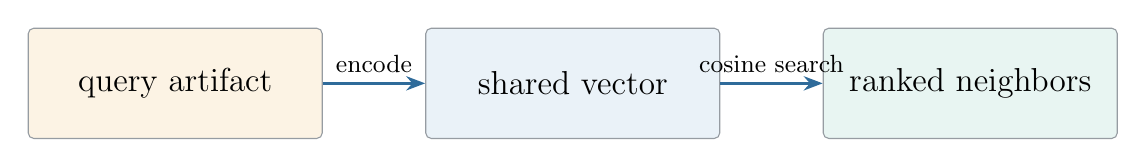
\begin{tikzpicture}[
    node distance=13mm,
    box/.style={draw=prgray!65,rounded corners=2pt,minimum height=14mm,
      text width=35mm,align=center,fill=white,font=\large},
    flow/.style={-{Stealth[length=2.4mm]},very thick,draw=prblue}
  ]
    \node[box,fill=prlightgold] (q) {query artifact};
    \node[box,fill=prlightblue,right=of q] (z) {shared vector};
    \node[box,fill=prlightteal,right=of z] (r) {ranked neighbors};
    \draw[flow] (q)--node[above,font=\small]{encode}(z);
    \draw[flow] (z)--node[above,font=\small]{cosine search}(r);
  \end{tikzpicture}
  \end{center}
  \vspace{5mm}
  \begin{columns}[T,onlytextwidth]
    \column{0.49\textwidth}
      \textbf{Example}\par
      \small Use an event log to find a related process tree or Petri net in a repository.
    \column{0.49\textwidth}
      \textbf{Interpretation}\par
      \small A high rank suggests a useful precedent. It does not certify behavioral equivalence.
  \end{columns}
  \source{ProcRosetta paper, cross-artifact retrieval task and application scenario.}
\end{frame}

% -----------------------------------------------------------------------------
\begin{frame}[t]{Decoding proposes valid process trees}
  \vspace{1mm}
  \paperfigure{figures/decoder}
  \vspace{2mm}
  \begin{columns}[T,onlytextwidth]
    \column{0.48\textwidth}
      \textbf{Guaranteed}\par
      \small Closed grammar, legal operator arity, permitted labels, Petri-net convertibility.
    \column{0.48\textwidth}
      \textbf{Not guaranteed}\par
      \small The candidate may still omit activities or encode the wrong behavior.
  \end{columns}
  \source{ProcRosetta paper, grammar-constrained decoder.}
\end{frame}

% -----------------------------------------------------------------------------
\begin{frame}[t]{Behavior families as training data}
  \vspace{4mm}
  \begin{center}
  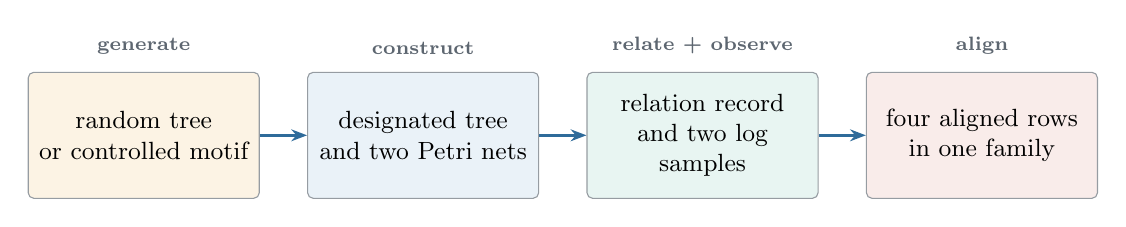
\begin{tikzpicture}[
    stage/.style={draw=prgray!65,rounded corners=2pt,minimum height=16mm,
      text width=27mm,align=center,font=\small},
    tag/.style={font=\scriptsize\bfseries,text=prgray},
    flow/.style={-{Stealth[length=2mm]},very thick,draw=prblue},
    node distance=6mm
  ]
    \node[stage,fill=prlightgold] (a) {random tree\\or controlled motif};
    \node[stage,fill=prlightblue,right=of a] (b) {designated tree\\and two Petri nets};
    \node[stage,fill=prlightteal,right=of b] (c) {relation record\\and two log samples};
    \node[stage,fill=prlightred,right=of c] (d) {four aligned rows\\in one family};
    \node[tag,above=1mm of a] {generate};
    \node[tag,above=1mm of b] {construct};
    \node[tag,above=1mm of c] {relate + observe};
    \node[tag,above=1mm of d] {align};
    \draw[flow] (a)--(b);
    \draw[flow] (b)--(c);
    \draw[flow] (c)--(d);
  \end{tikzpicture}
  \end{center}
  \vspace{5mm}
  \begin{columns}[c,onlytextwidth]
    \column{0.34\textwidth}
      {\fontsize{23}{26}\selectfont\bfseries\color{prblue}15,360}\par
      \small behavior families
    \column{0.34\textwidth}
      {\fontsize{23}{26}\selectfont\bfseries\color{prteal}61,440}\par
      \small aligned rows
    \column{0.32\textwidth}
      \textbf{Split as a family}\par
      \small All realizations and observations stay together.
  \end{columns}
  \source{Adapted from the ProcRosetta corpus-construction figure and dataset table.}
\end{frame}

% -----------------------------------------------------------------------------
\begin{frame}[t]{A family is the supervision unit}
  \vspace{0mm}
  \keyline{A family organizes comparisons; it does not declare equivalence.}
  \vspace{2mm}
  \centering
  \large
  \textbf{1 tree target + 2 net realizations + 2 log observations}
  $\longrightarrow$ \textbf{4 aligned rows}
  \par\vspace{2mm}

  \scriptsize
  \renewcommand{\arraystretch}{1.08}
  \setlength{\tabcolsep}{4pt}
  \begin{tabular}{@{}>{\raggedright\arraybackslash}p{0.36\textwidth}
                      >{\raggedright\arraybackslash}p{0.55\textwidth}@{}}
    \toprule
    Relationship & Learning signal and effect \\
    \midrule
    Row + tree target & \textbf{Reconstruction:} learn one common output. \\
    Two log samples & \textbf{Observation consistency:} ignore sampling variation. \\
    Same language + partial order & \textbf{Strong positive:} align tightly. \\
    Same language, different partial order & \textbf{Hierarchical relation:} stay close, but keep concurrency distinct. \\
    \bottomrule
  \end{tabular}
  \par\vspace{2mm}
  \small\textbf{Across families:} behavior distance $d_B$ shapes geometry and ranking.
  \source{Adapted from the ProcRosetta paper, ``From generated relationships to learning signals.''}
\end{frame}

% -----------------------------------------------------------------------------
\begin{frame}[t]{Training complexity grows in stages}
  \vspace{-1mm}
  \paperfigure{figures/training}
  \vspace{-1mm}
  \centering
  \small
  \begin{tabular}{@{}>{\bfseries}lcl@{}}
    \textcolor{prgold}{Simple} & epochs 1--5 & basic grammar and alignment \\
    \textcolor{prteal}{Medium mix} & epochs 6--10 & deeper structures + simple rehearsal \\
    \textcolor{prred}{Complex mix} & epochs 11--17 & target range + earlier rehearsal \\
  \end{tabular}
  \par\vspace{0mm}
  \source{ProcRosetta paper, curriculum schedule and training chart.}
\end{frame}

% -----------------------------------------------------------------------------
\begin{frame}[t]{The analyst stays in the loop}
  \vspace{0mm}
  \paperfigure{figures/workflow}
  \vspace{2mm}
  \keyline{Retrieve first; propose only when useful; validate before acceptance.}
  \source{ProcRosetta paper, intended application workflow.}
\end{frame}

% -----------------------------------------------------------------------------
\begin{frame}[t]{One tool, three work areas}
  \vspace{1mm}
  \begin{columns}[T,onlytextwidth]
    \column{0.325\textwidth}
      \centering
      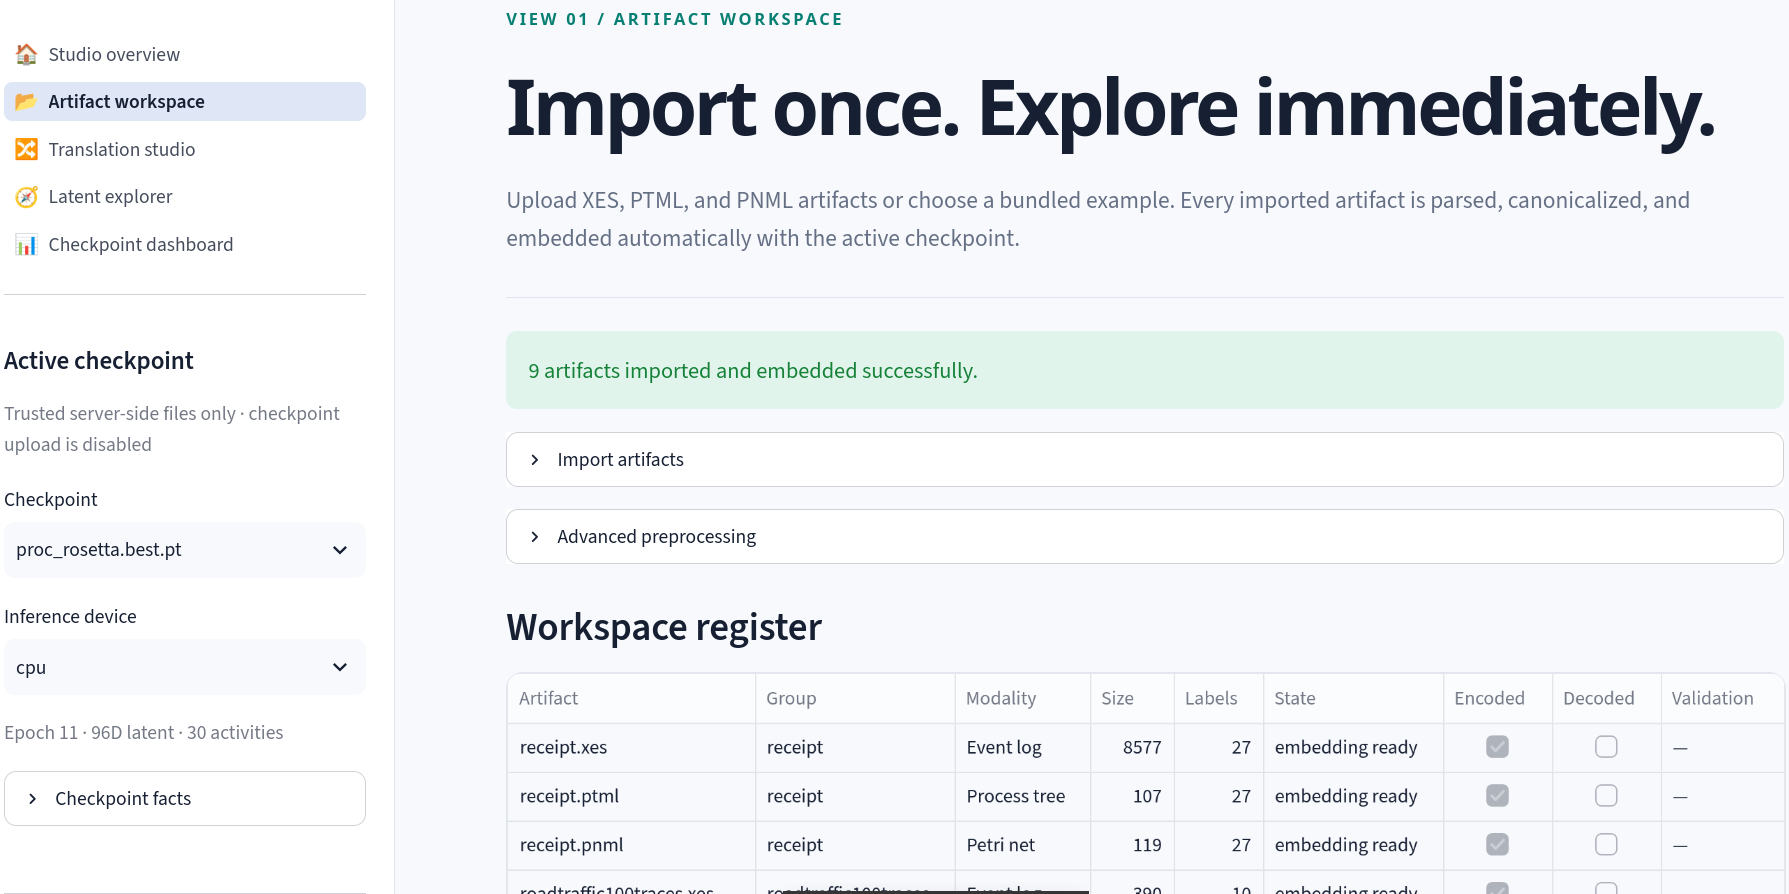
\includegraphics[width=\linewidth]{screenshots/rosetta-pm-artifact-workspace.png}\par
      \vspace{2mm}\textbf{1. Load}\par
      {\small Register and inspect evidence.}
    \column{0.325\textwidth}
      \centering
      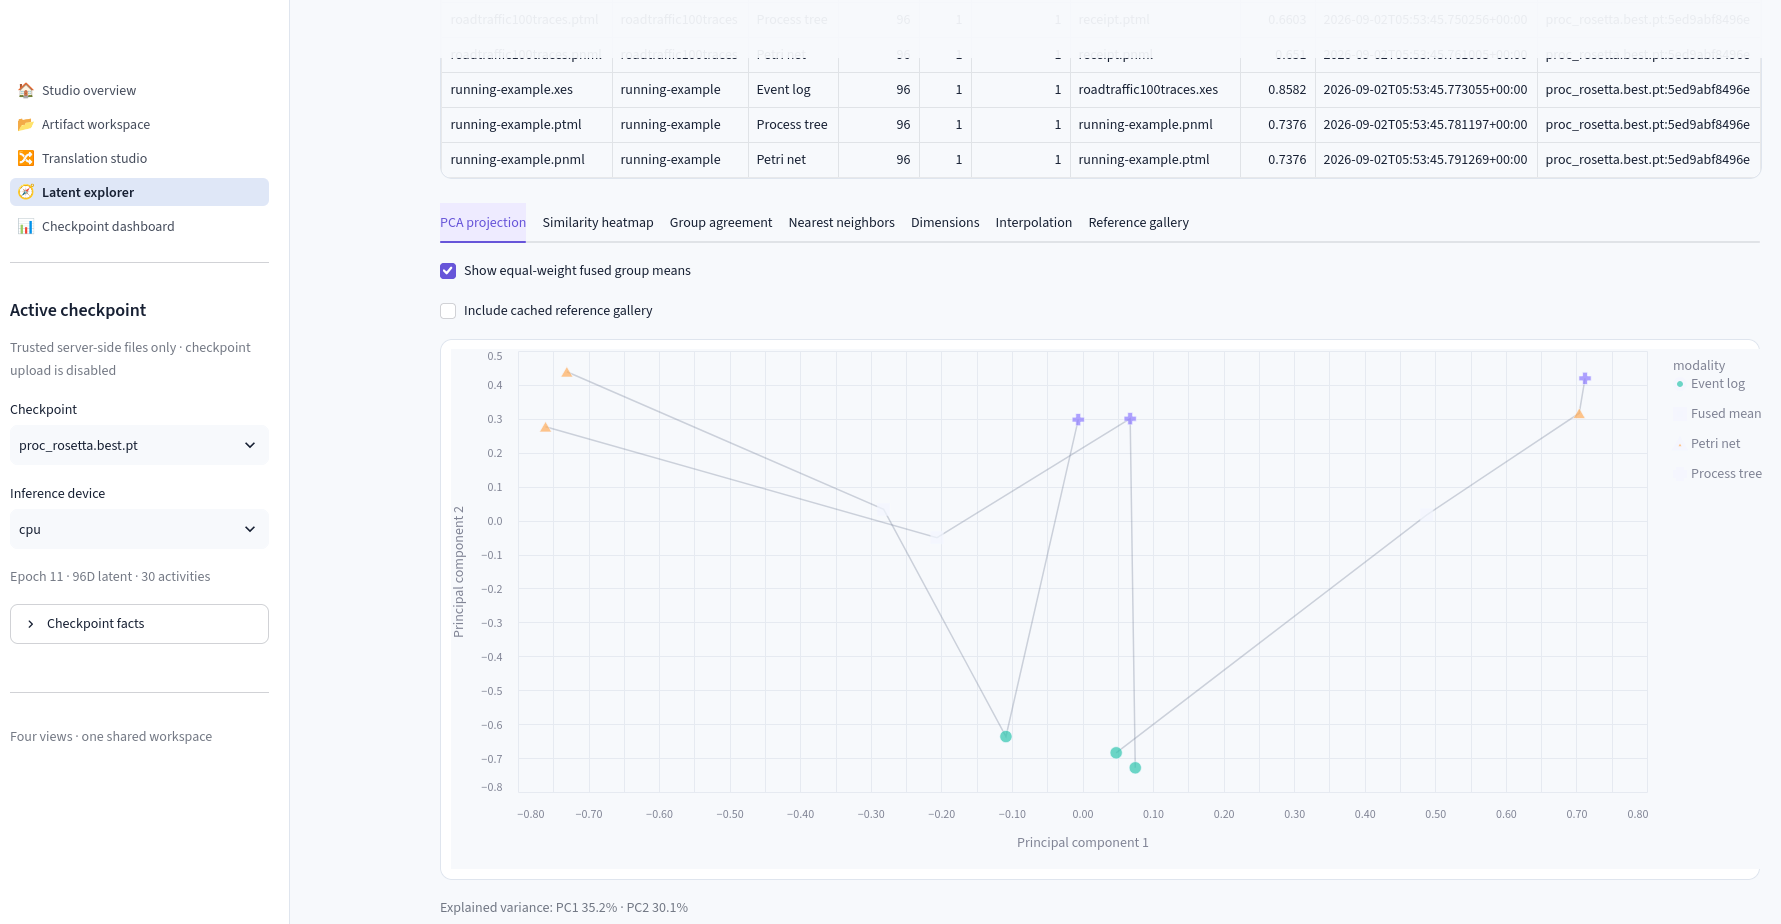
\includegraphics[width=\linewidth]{screenshots/rosetta-pm-latent-explorer.png}\par
      \vspace{2mm}\textbf{2. Compare}\par
      {\small Inspect similarities and neighbors.}
    \column{0.325\textwidth}
      \centering
      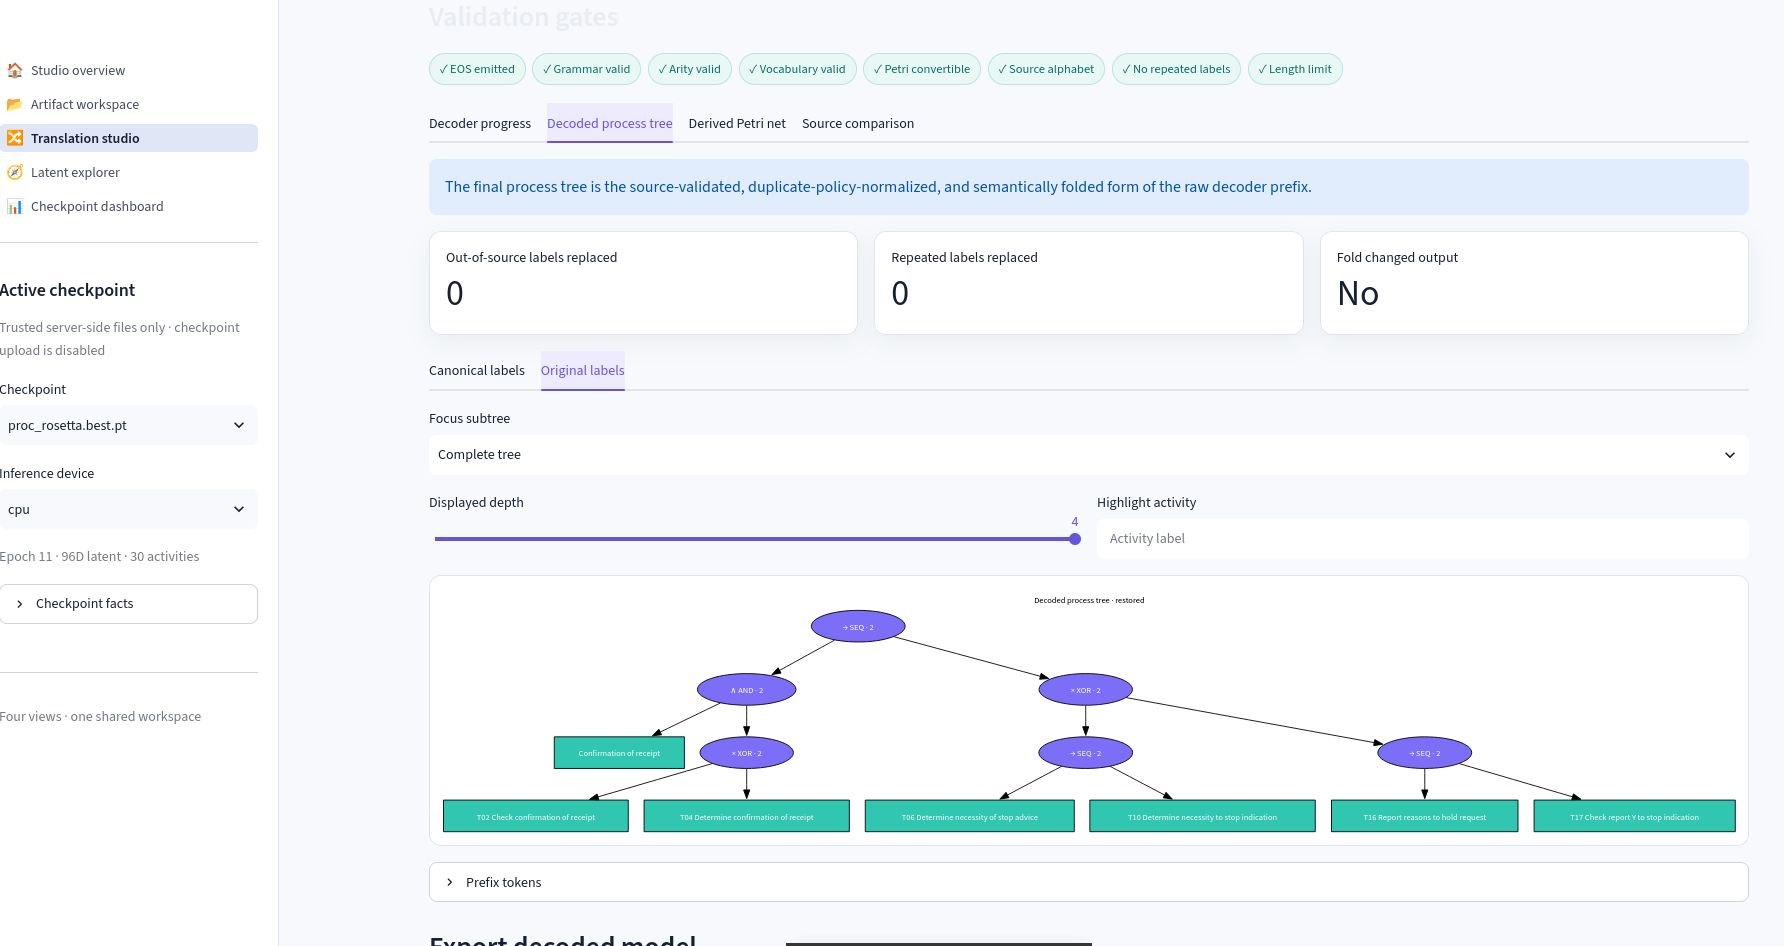
\includegraphics[width=\linewidth]{screenshots/rosetta-pm-translation-studio.png}\par
      \vspace{2mm}\textbf{3. Propose}\par
      {\small Decode, validate, and export.}
  \end{columns}
  \vspace{3mm}
  \centering
  \large\textbf{rosetta-pm.app}\quad\color{prgray}records artifacts, checkpoints, settings, and validation.
  \source{ProcRosetta paper, reference-interface screenshots.}
\end{frame}

% -----------------------------------------------------------------------------
\begin{frame}[t]{The learned geometry gets stronger}
  \vspace{-1mm}
  \paperfigure{figures/geometry-bars}
  \vspace{-1mm}
  \keyline{Fused embedding: Spearman $\rho$ rises from 0.577 to 0.791 as complexity grows.}
  \source{ProcRosetta paper, behavioral-ordering results on the fixed 48-family subset.}
\end{frame}

% -----------------------------------------------------------------------------
\begin{frame}[t]{Retrieval succeeds in all directions}
  \vspace{1mm}
  \begin{columns}[c,onlytextwidth]
    \column{0.74\textwidth}
      \centering
      \footnotesize
      \setlength{\tabcolsep}{4.2pt}
      \begin{tabular}{@{}lccc@{}}
        \toprule
        Direction & \texttt{simple} & \texttt{medium} & \texttt{complex} \\
        \midrule
        PN $\rightarrow$ log  & .703 / .755 & .766 / .799 & .828 / .855 \\
        PN $\rightarrow$ tree & .828 / .862 & .828 / .862 & .828 / .862 \\
        Log $\rightarrow$ PN  & .750 / .805 & .719 / .785 & .750 / .801 \\
        Log $\rightarrow$ tree & .656 / .705 & .656 / .705 & .688 / .730 \\
        Tree $\rightarrow$ PN & .812 / .867 & .875 / .908 & .875 / .908 \\
        Tree $\rightarrow$ log & \best{.875 / .905} & \best{.875 / .905} & \best{.875 / .905} \\
        \bottomrule
      \end{tabular}
      \par\vspace{1mm}
      {\scriptsize Recall@1 / MRR; higher is better.}
    \column{0.23\textwidth}
      {\fontsize{17}{20}\selectfont\bfseries\color{prteal}0.656--0.875}\par
      \small Recall@1 range\par\vspace{5mm}
      {\fontsize{20}{23}\selectfont\bfseries\color{prgray}.0625}\par
      \small random Recall@1
  \end{columns}
  \vspace{2mm}
  \centering
  \small Hardest direction: finite event log $\rightarrow$ explicit process tree.
  \source{ProcRosetta paper, cross-artifact retrieval table; 16 families per level.}
\end{frame}

% -----------------------------------------------------------------------------
\begin{frame}[t]{Valid does not mean faithful}
  \vspace{0mm}
  \keyline{Every output is grammar-valid; event-log exact match is 0\% at every level.}
  \vspace{1mm}
  \centering
  \footnotesize
  \setlength{\tabcolsep}{4.2pt}
  \begin{tabular}{@{}llrrrr@{}}
    \toprule
    Level & Method & Evaluable & Fitness & Precision & F1 \\
    \midrule
    \multirow{2}{*}{\texttt{simple}}
      & \model & 78.1\% & .702 & .654 & .666 \\
      & Inductive Miner & 100\% & 1.000 & .992 & \best{.996} \\
    \midrule
    \multirow{2}{*}{\texttt{medium}}
      & \model & 75.0\% & .709 & .663 & .669 \\
      & Inductive Miner & 100\% & 1.000 & .986 & \best{.992} \\
    \midrule
    \multirow{2}{*}{\texttt{complex}}
      & \model & 71.9\% & .691 & .639 & .649 \\
      & Inductive Miner & 100\% & 1.000 & .907 & \best{.938} \\
    \bottomrule
  \end{tabular}
  \par\vspace{3mm}
  \small For event-log process discovery, the specialized baseline remains substantially stronger.
  \source{ProcRosetta paper, candidate-generation and process-discovery result tables.}
\end{frame}

% -----------------------------------------------------------------------------
\begin{frame}[t]{Retrieve, propose, then validate}
  \vspace{5mm}
  \begin{center}
  
\begin{tikzpicture}[
    processstep/.style={font=\fontsize{19}{22}\selectfont\bfseries,align=center},
    flow/.style={-{Stealth[length=3mm]},very thick,draw=prblue}
  ]
    \node[processstep,text=prblue] (a) {Retrieve};
    \node[processstep,text=prgold,right=27mm of a] (b) {Propose};
    \node[processstep,text=prteal,right=27mm of b] (c) {Validate};
    \draw[flow] (a)--(b);
    \draw[flow] (b)--(c);
  \end{tikzpicture}
  \end{center}
  \vspace{6mm}
  \begin{columns}[T,onlytextwidth]
    \column{0.47\textwidth}
      \textbf{What works now}\par
      \small A single representation supports cross-artifact neighborhood search across logs, trees, and nets.
    \column{0.47\textwidth}
      \textbf{What remains open}\par
      \small Behaviorally faithful generation, real aligned benchmarks, and behavior-disjoint evaluation.
  \end{columns}
  \vspace{5mm}
  \begin{center}
    \Large\bfseries\color{prnavy}Alignment is stronger than translation.
  \end{center}
  \source{ProcRosetta paper, discussion and conclusion.}
\end{frame}

\end{document}
